\subsubsection*{Implementación de modelos de XAI para la interpretabilidad del modelo Wav2Vec2 fine-tuneado}

Ahora que tenemos el resultado del modelo (el Wav2Vec2 fine-tuneado), vamos a explicar que características y que parte del espectrograma de Mel del audio son las más influyentes y en que sentido.

Sin embargo ahora nos encontramos con el problema principal de este modelo que es que como entrada recibe un embedding, entonces, no podemos aplicar técnicas de XAI directamente al modelo. Otro problema que tenemos es que el código que tenemos de extracción de características saca muchísimas características y de ciertas características no solo saca un valor escalar sino que también saca un vector con sus valores en cada instante.

Para solucionar estos problemas hemos hecho dos cosas. La primera es que agruparemos las características en cinco grupos en función de sus características y lo que representan. Con esto nos quedan las siguientes agrupaciones:

\begin{enumerate}
 \item Energía: rms, silence ratio, zcr, skewness, kurtosis. Este grupo son las características que se centran en la energía del audio.
 \item Espectrales: spectral centroid, spectral bandwidth, spectral rolloff, spectral flatness, hnr. Este grupo son las características que miden la distribución de la energía en el ámbito de la frecuencia.
 \item Pitch: pitch mean, pitch std. Este grupo son las características %falta completar
 \item Formantes:  f1 mean, f2 mean, f3 mean. Este grupo son las características que describen la estructura vocal.
 \item MFCC: mfcc1 mean, mfcc2 mean,  mfcc3 mean, mfcc4 mean,  mfcc5 mean, mfcc6 mean,  mfcc7 mean, mfcc8 mean,  mfcc9 mean, mfcc10 mean,  mfcc11 mean, mfcc12 mean,  mfcc13 mean. Este grupo de características capturan %falta completar
	\end{enumerate}

La segunda cosa que se ha hecho ha sido desarrollar modelos sencillos que imiten el comportamiento del modelo. Para esto hemos hecho 6 modelos distintos. Cinco de ellos son regresiones logísticas, uno para cada grupo de características y una CNN muy simple para los espectrogramas.

Una vez tenemos los surrogate models hechos, ahora les vamos a aplicar técnicas de ia explicable. La primera técnica que aplicaremos a cada modelo de regresión es el Shap. Para cada modelo, esta técnica nos sacará dos gráficas, la primera es el impacto general de cada característica en la respuesta del modelo	y la segunda es el impacto de cada característica para un audio concreto. Con esto, vamos a ir explicando modelo por modelo.

\begin{enumerate}
 \item Energía: En este modelo podemos ver como la kurtosis y el silence ratio son las características que más influyen mientras que el rms tiene una influencia nula en la predicción. 
 
 \begin{figure}[H]
	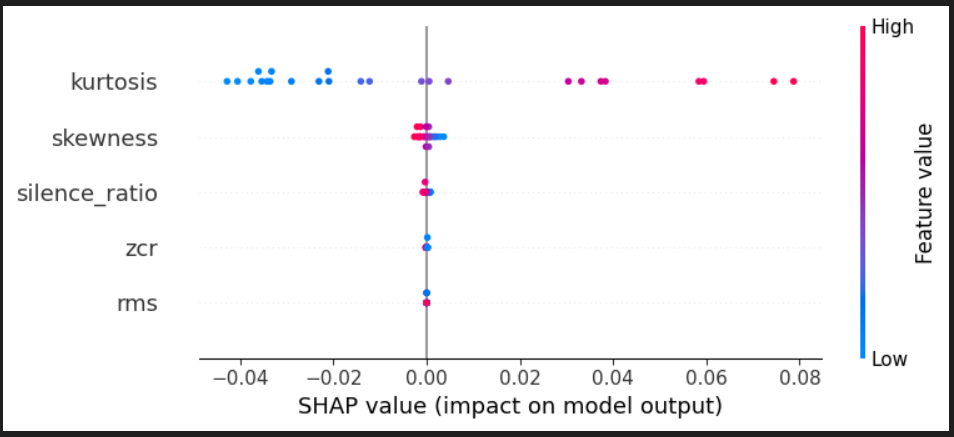
\includegraphics[width=\textwidth]{imagenes/Influencia_caracteristicas_energia_wav2vec2.png}
	\caption{Influencia general de las características.}
	\label{fig:Wav2Vec2}
 \end{figure}
 
En este ejemplo concreto tenemos que tener en cuenta que los valores del audio para las características de la energía son:
 
 %Hacerlo tabla
 \begin{enumerate}
  \item rms: 0,019 - Esto nos indica que el audio tiene un volumen muy bajo, algo por debajo del rango típico de voz estándar pero coherente con voces sin procesar.
\item silence\_ratio: 0.760 - Esto nos dice que el 76\% del audio es silencio.
\item skewness: -0.494 - Esto muestra que el audio tiene una ligera asimetría negativa.
  \item skewness: -0,494 - Esto muestra que el audio tiene una ligera asimetría negativa.
  \item kurtosis: 28,548 - Esto es un curtosis extremadamente alta que encaja con voz intermitente o silencios largos junto con palabras puntuales.
 \end{enumerate}
 
 \begin{figure}[H]
	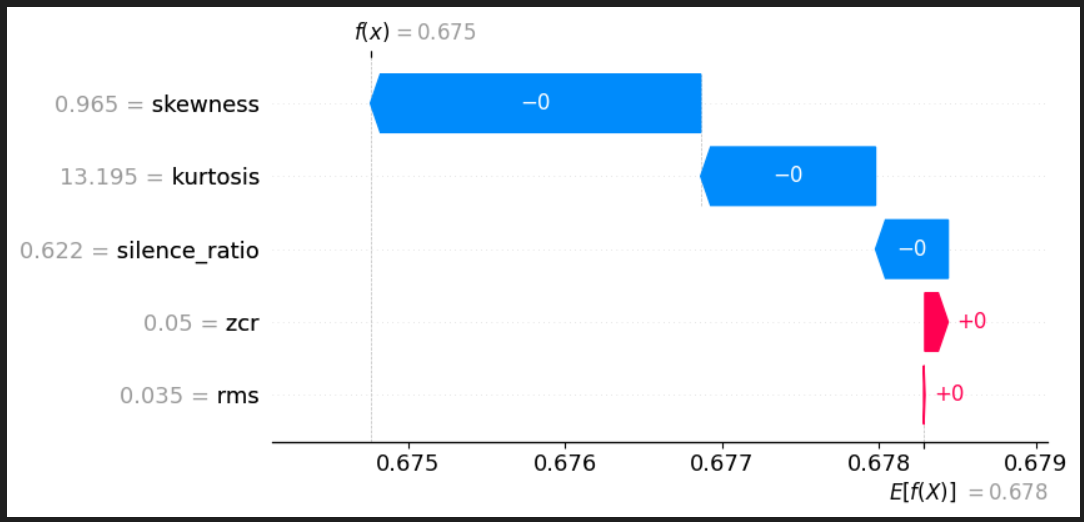
\includegraphics[width=\textwidth]{imagenes/Influencia_caracteristicas_energia_instancia_wav2vec2.png}
	\caption{Ejemplo concreto.}
	\label{fig:Wav2Vec2}
 \end{figure}
 
 A la vista de la imagen podemos ver que ninguna de las características influye demasiado en la predicción pero si que se mantiene el orden global y se puede ver con cuanta fuerza influirían y en que dirección. En este caso y por la fuerza que se le presupone a las características, este audio es más real que generado. 

 \item Espectrales: En este modelo podemos ver como el spectral centroid es la característica dominante aunque seguida de cerca por el spectral rolloff y el spectral bandwidth. También se puede apreciar que el spectral flatness no tiene influencia en la predicción.
 
 \begin{figure}[H]
	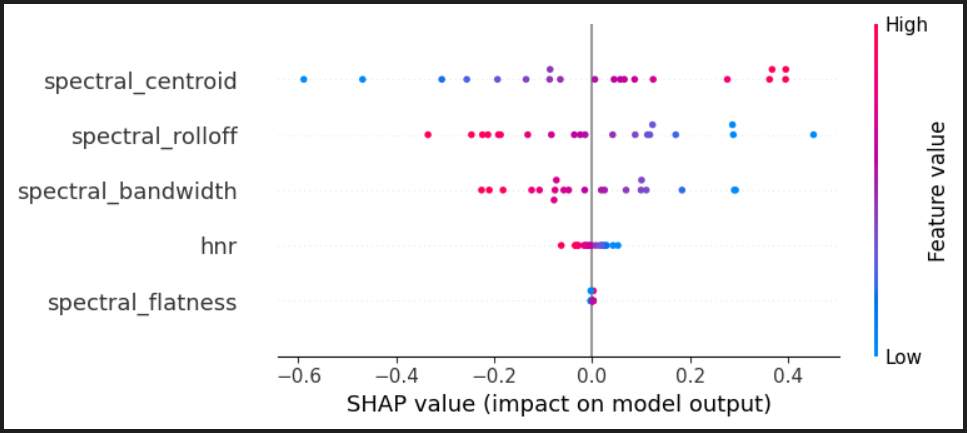
\includegraphics[width=\textwidth]{imagenes/Influencia_caracteristicas_espectrales_wav2vec2.png}
	\caption{Influencia general de las características.}
	\label{fig:Wav2Vec2}
 \end{figure}

En este ejemplo concreto tenemos que tener en cuenta que los valores del audio para las características espectrales son:

%Hacerlo tabla
 \begin{enumerate}
  \item spectral centroid: 1636,524 - Presenta un centro de masa típico de voces habladas.
  \item spectral bandwidth: 1590,950 - Esto indica una dispersión moderada del espectro lo que es típico de voces complejas.
  \item spectral rolloff: 2916,263 - Este es un rolloff típico de voces con consonantes.
  \item spectral flatness: 0,034 - Esto nos muestra que es una señal altamente tonal, es decir, sin ruido.
  \item hnr: 11,754 - Presenta un valor típico para las voces (entre 10 y 20)
 \end{enumerate}

 \begin{figure}[H]
	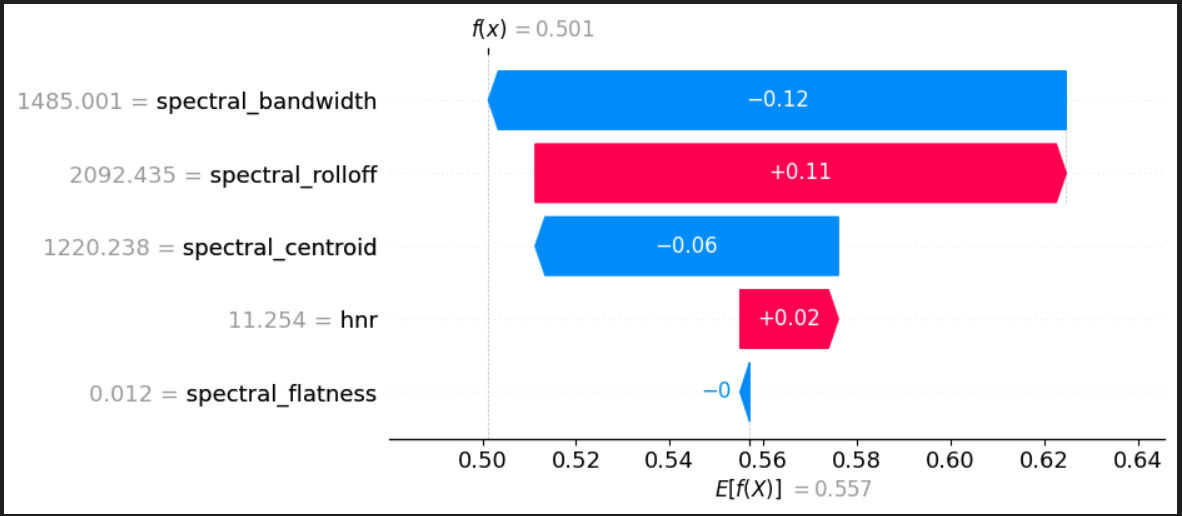
\includegraphics[width=\textwidth]{imagenes/Influencia_caracteristicas_espectrales_instancia_wav2vec2.png}
	\caption{Ejemplo concreto.}
	\label{fig:Wav2Vec2}
 \end{figure}
 
 A la vista de la imagen podemos ver como según estas características, este audio es más probable que sea real. 
 
 \item Pitch: En este modelo hay un claro dominio por parte del pitch std en comparación con el pitch mean.
 
 \begin{figure}[H]
	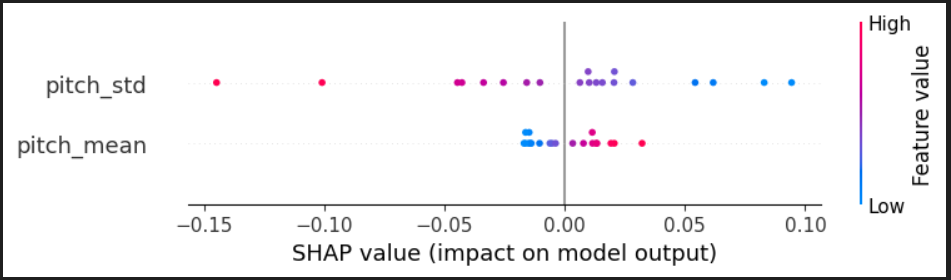
\includegraphics[width=\textwidth]{imagenes/Influencia_caracteristicas_pitch_wav2vec2.png}
	\caption{Influencia general de las características.}
	\label{fig:Wav2Vec2}
 \end{figure}

En este ejemplo concreto tenemos que tener en cuenta que los valores del audio para el pitch son:

%Hacerlo tabla
 \begin{enumerate}
  \item pitch std: 55,340 - Este valor muestra la variabilidad del pitch siendo en este caso un valor de variabilidad alto.
  \item pitch mean: 266,192 - Este es un valor alto para el pitch lo que denota voces agudas
 \end{enumerate}
 
 \begin{figure}[H]
	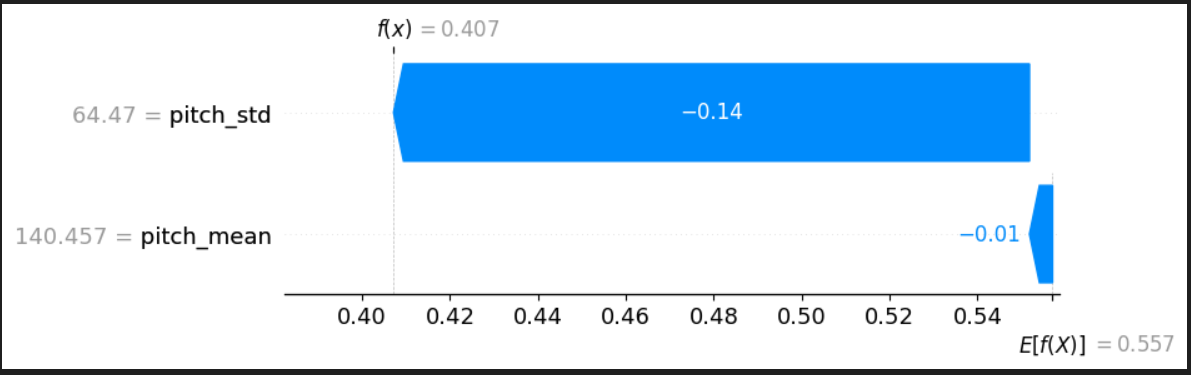
\includegraphics[width=\textwidth]{imagenes/Influencia_caracteristicas_pitch_instancia_wav2vec2.png}
	\caption{Ejemplo concreto.}
	\label{fig:Wav2Vec2}
 \end{figure}
 
A la vista de la imagen podemos ver ambas características empujan al modelo a decidir que este audio es real.
 
 \item Formantes: En este modelo la f1 y la f3 tienen una influencia similar y muy superior a la de f2.
 
 \begin{figure}[H]
	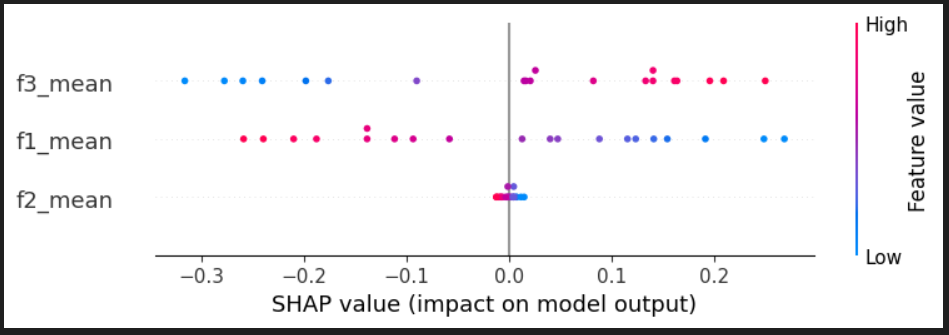
\includegraphics[width=\textwidth]{imagenes/Influencia_caracteristicas_formants_wav2vec2.png}
	\caption{Influencia general de las características.}
	\label{fig:Wav2Vec2}
 \end{figure}

En este ejemplo concreto tenemos que tener en cuenta que los valores del audio para las formantes son:

%Hacerlo tabla
 \begin{enumerate}
  \item f1 mean: 1001,886 - Este es un valor alta de f1, típico de las vocales abiertas (A,E,O).
  \item f2 mean: 2104,974 - Este es un valor típico de las vocales frontales o anteriores (E,I). Las vocales posteriores tendrían valores menores de 1200.
  \item f3 mean: 3271,627 - Este valor muestra una voz con un timbre bastante claro y resonante típico de voces femeninas o voces masculinas poco graves.
 \end{enumerate}
 
 \begin{figure}[H]
	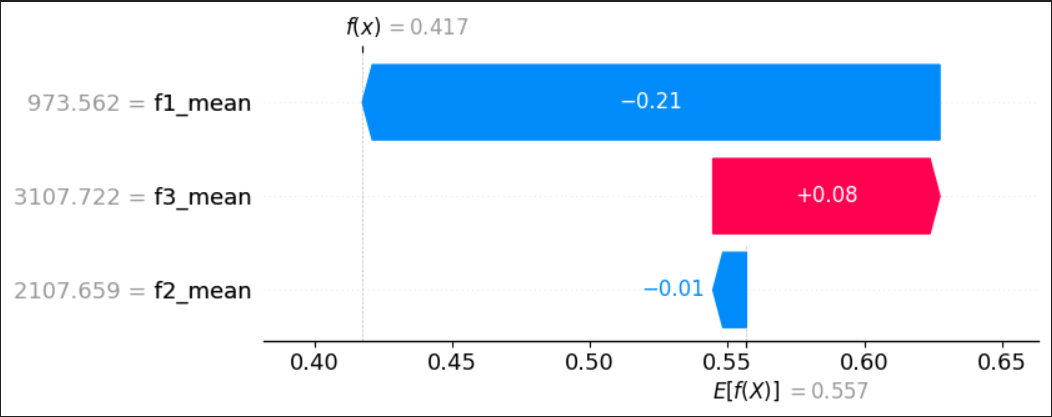
\includegraphics[width=\textwidth]{imagenes/Influencia_caracteristicas_formants_instancia_wav2vec2.png}
	\caption{Ejemplo concreto.}
	\label{fig:Wav2Vec2}
 \end{figure} 
 
 En la imagen se puede apreciar como la f1 es la que más tira de la predicción hacia la clase real mientras que la f3 en bastante menos medida lo hace hacia la clase generado.
 
 \item MFCC: En este modelo se observa como los coeficientes cepstrales de Mel 5,6 y 7 son los que más influyen mientras que los coeficientes 1,13 y 12 son los que menos influyen.
 
  \begin{figure}[H]
	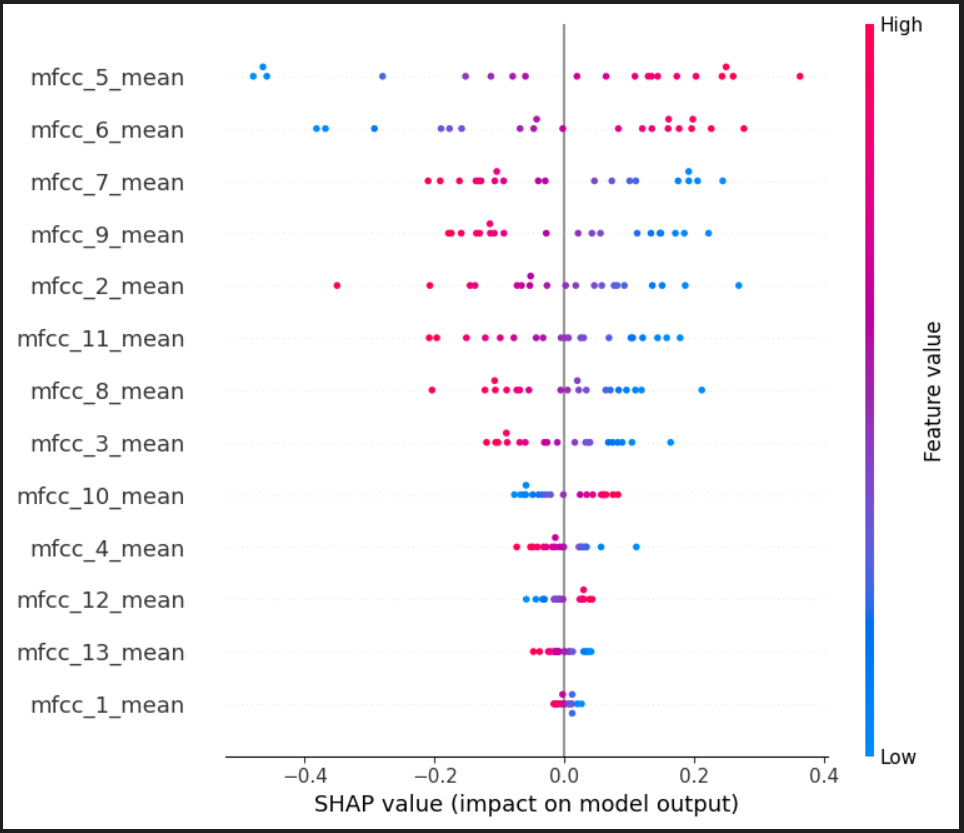
\includegraphics[width=\textwidth]{imagenes/Influencia_caracteristicas_MFCC_wav2vec2.png}
	\caption{Influencia general de las características.}
	\label{fig:Wav2Vec2}
 \end{figure}

En este ejemplo concreto tenemos que tener en cuenta que los valores del audio para las características espectrales son:

%Hacerlo tabla
 \begin{enumerate}
  \item mfcc1 mean: -456,798 - Es un valor bastante bajo, típico de audios con pausas frecuentes.
  \item mfcc2 mean: 45,541 - Esto indica que es una voz con más énfasis en fonemas graves y medios.
  \item mfcc3 mean: 2,062 - Esto nos dice que el espectro es bastante equilibrado.
  \item mfcc4 mean: 16,164 - Esto nos habla de la presencia de consonantes agudas.
  \item mfcc5 mean: -1,455 - Esto muestra que es una voz natural y sin exceso de brillo.
  \item mfcc6 mean: 12,418 - Esto indica que la voz hablada es clara.
  \item mfcc7 mean: 4,943 - Esto indica que la señal es estable y natural.
  \item mfcc8 mean: 10,452 - Esto nos dice que la voz presenta consonantes articuladas.
  \item mfcc9 mean: 8,349 - Esto indica que la voz es clara y con información armónica preservada.
  \item mfcc10 mean: 3,038 - Esto muestra que es voz natural, es decir, sin ruido blanco.
  \item mfcc11 mean: 10,387 - Esto refuerza la claridad de la voz.
  \item mfcc12 mean: 12,444 - Esto nos habla de que es voz articulada.
  \item mfcc13 mean: 10,578 - Esto nos dice que la voz no presenta distorsión.
 \end{enumerate}
 
 \begin{figure}[H]
	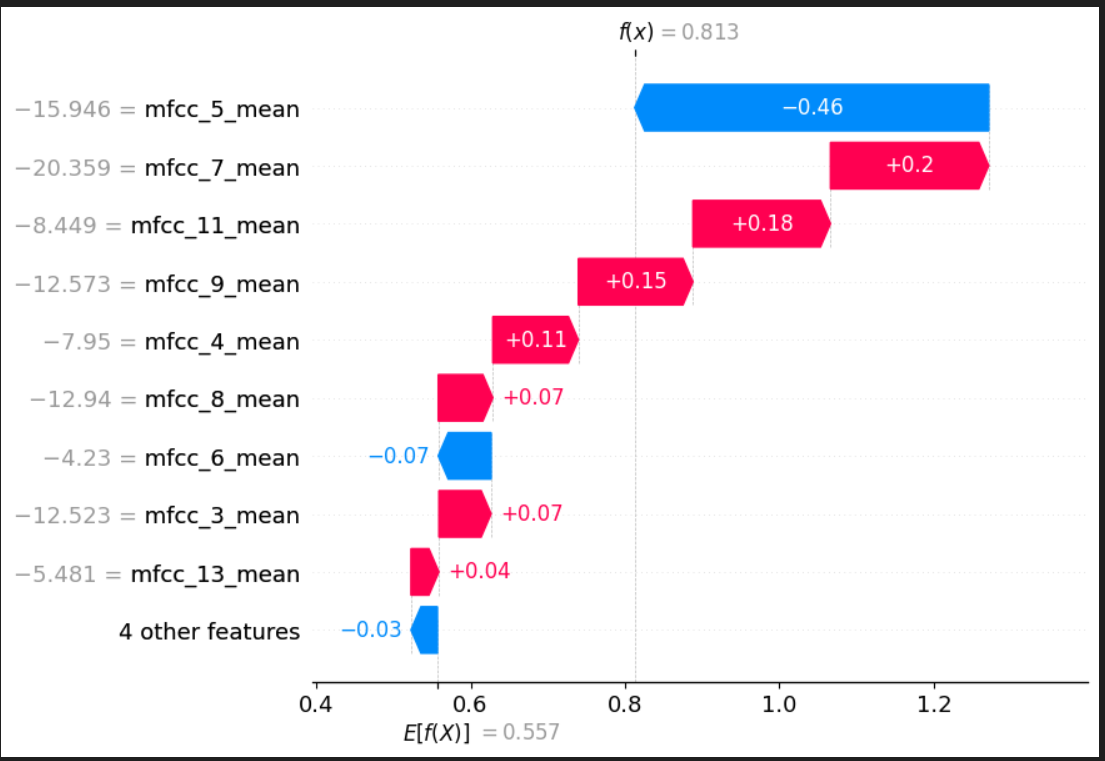
\includegraphics[width=\textwidth]{imagenes/Influencia_caracteristicas_MFCC_instancia_wav2vec2.png}
	\caption{Ejemplo concreto.}
	\label{fig:Wav2Vec2}
 \end{figure}
 
 En la imagen podemos apreciar como este grupo de características en conjunto empujan la predicción hacia la clase generado siendo que lo que la mfcc5 empuja hacia la clase real se ve contrarrestado por las mfcc7, mfcc11 y mfcc9.
 
	\end{enumerate}

Ahora para las características, buscando también algo que complemente la explicación del Shap, vamos a usar Lime para explicar los mismos modelos y la misma instancia particular.

\begin{enumerate}
 \item Energía: En este modelo podemos ver como la kurtosis es la única característica que tiene un impacto relevante en la predicción del modelo. 
 
 \begin{figure}[H]
	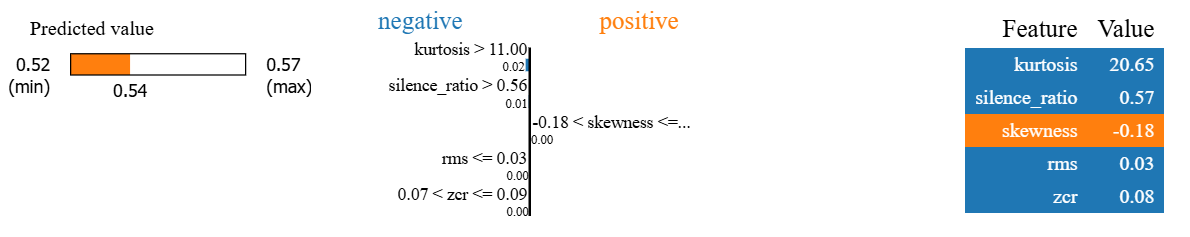
\includegraphics[width=\textwidth]{imagenes/Influencia_caracteristicas_energia_lime_wav2vec2.png}
	\caption{Influencia general de las características.}
	\label{fig:Wav2Vec2}
 \end{figure}

 \item Espectrales: En este modelo podemos ver como todas las características tienen algo de impacto, sin embargo predominan claramente el espectral bandwidth y el espectral centroid hacia reducir la predicción y el espectral rolloff hacia aumentarla.
 
 \begin{figure}[H]
	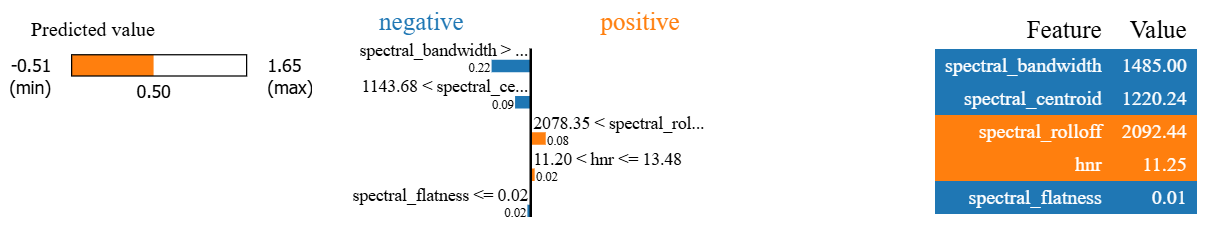
\includegraphics[width=\textwidth]{imagenes/Influencia_caracteristicas_espectrales_lime_wav2vec2.png}
	\caption{Influencia general de las características.}
	\label{fig:Wav2Vec2}
 \end{figure}
 
 \item Pitch: En este modelo se ve como el pitch std influye más que el pitch mean. Ambas características empujan la predicción hacia abajo.
 
 \begin{figure}[H]
	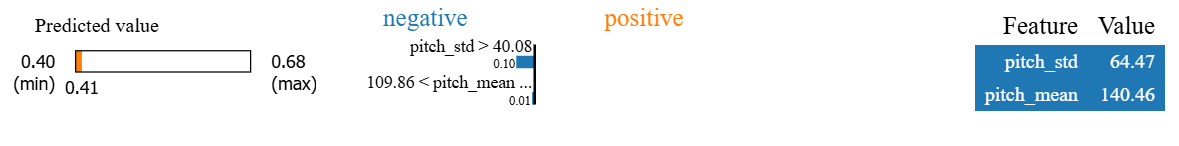
\includegraphics[width=\textwidth]{imagenes/Influencia_caracteristicas_pitch_lime_wav2vec2.png}
	\caption{Influencia general de las características.}
	\label{fig:Wav2Vec2}
 \end{figure}
 
 \item Formantes: En este modelo la f1 domina sobre las demás siendo la que más empuja la predicción hacia alguna dirección, en este caso, contribuye a reducirla mientras que la f3 la empuja hacia arriba aunque con menos fuerza de lo que la f1 lo hace hacia abajo.
 
 \begin{figure}[H]
	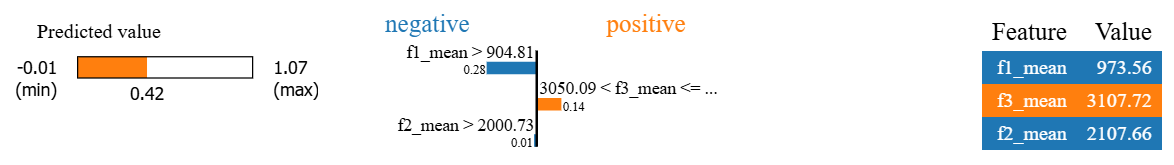
\includegraphics[width=\textwidth]{imagenes/Influencia_caracteristicas_formants_lime_wav2vec2.png}
	\caption{Influencia general de las características.}
	\label{fig:Wav2Vec2}
 \end{figure}
 
 \item MFCC: En este modelo los coeficientes 5,7,9 y 11 son los que más influyen en las decisiones del modelo siendo que el 5 es el coeficiente que más disminuye la predicción mientras que el 7, el 9 y el 11 son los que más la aumentan.
 
  \begin{figure}[H]
	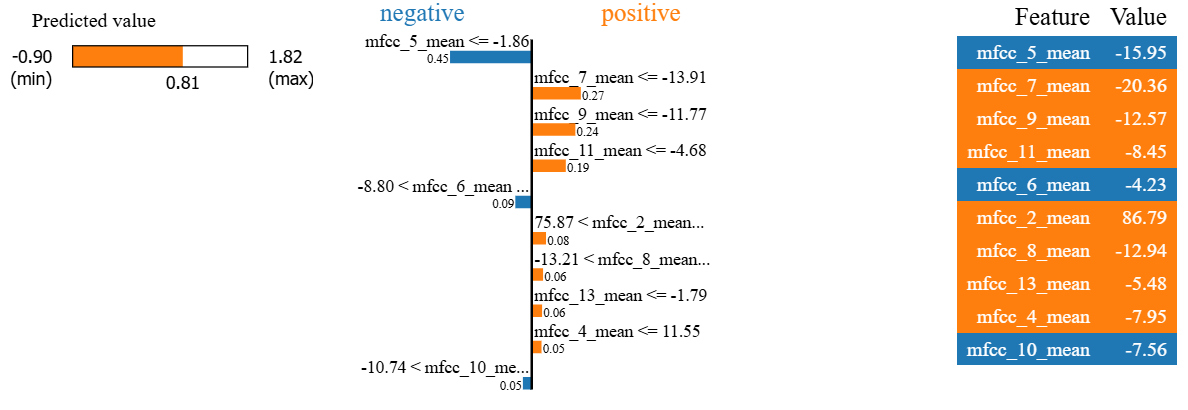
\includegraphics[width=\textwidth]{imagenes/Influencia_caracteristicas_MFCC_lime_wav2vec2.png}
	\caption{Influencia general de las características.}
	\label{fig:Wav2Vec2}
 \end{figure}
 
	\end{enumerate}

Ahora que ya tenemos tanto el Shap como el Lime de todas las características de los audios, vamos a agregar los resultados de los cinco modelos para ver de forma general cuales son las características más influyentes a la hora de clasificar los audios en reales o generados.

Para esta tarea se ha hecho lo siguiente, primero calculamos la importancia promedio de cada característica usando sus valores Shap, luego calculamos la importancia de cada grupo de características y con esto podemos promediar la importancia de cada característica entre todos los grupos de características. Por último los ordenamos de mayor a menor importancia y los mostramos.

\begin{figure}[H]
	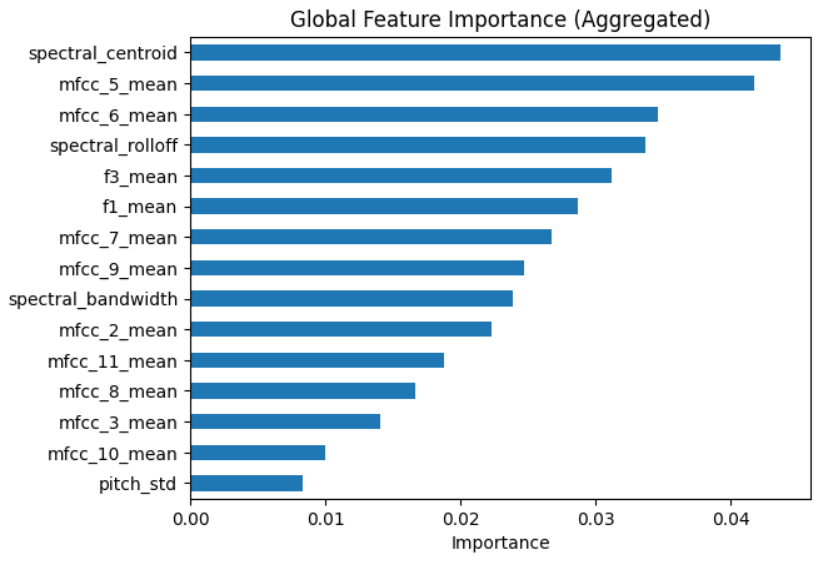
\includegraphics[width=\textwidth]{imagenes/Ranking_caracteristicas_shap_wav2vec2.png}
	\caption{Influencia general de las características.}
	\label{fig:Wav2Vec2}
\end{figure}

En esta gráfica podemos ver las 15 características más importantes para la predicción destacando sobre todo el centroide espectral y el 5º coeficiente cepstral de Mel.

Para Lime hacemos exactamente lo mismo.

\begin{figure}[H]
	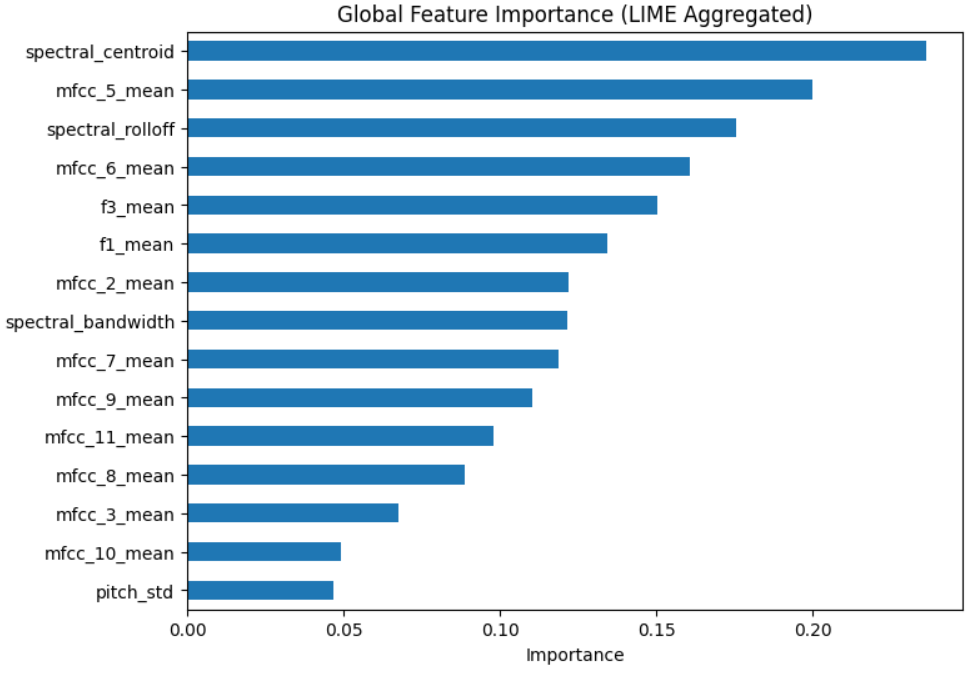
\includegraphics[width=\textwidth]{imagenes/Ranking_caracteristicas_lime_wav2vec2.png}
	\caption{Influencia general de las características.}
	\label{fig:Wav2Vec2}
\end{figure}

En esta gráfica destacan las mismas características que en la de Shap pero con ligeras variaciones de posición entre ellas.

Para acabar con la explicación de las características, vamos a juntar ambas explicaciones en una sola combinada para obtener el orden global de influencia de las características. Este orden será calculado haciendo la media aritmética de su importancia en shap y lime.

\begin{figure}[H]
	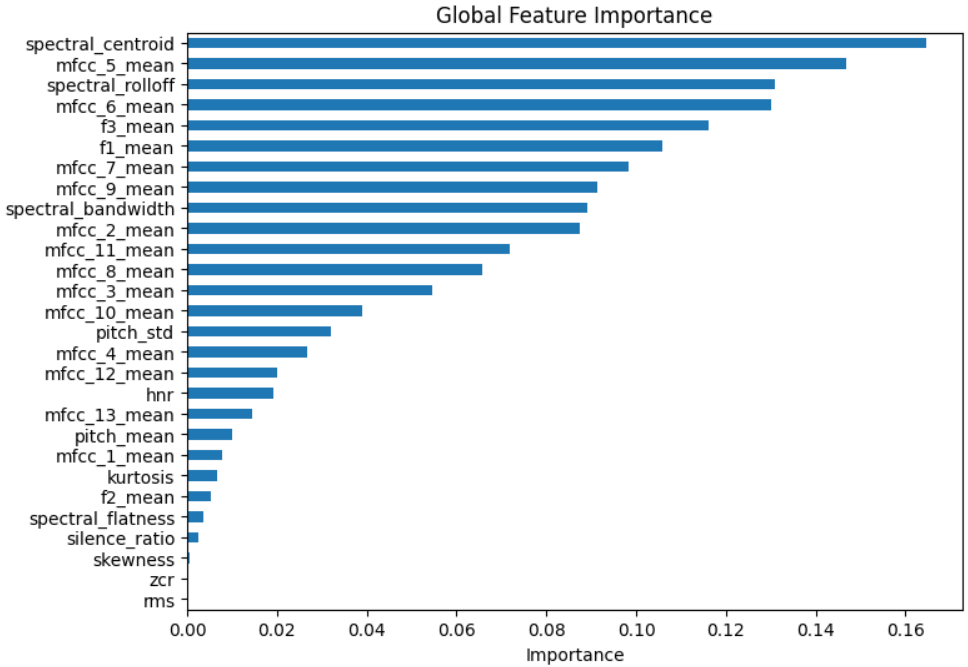
\includegraphics[width=\textwidth]{imagenes/Ranking_caracteristicas_final_wav2vec2.png}
	\caption{Influencia general de las características.}
	\label{fig:Wav2Vec2}
\end{figure}

En esta gráfica combinada podemos ver el ranking global de las características según su importancia.

Ahora pasamos al sexto surrogate model, una CNN muy simple que se compone solo de una capa convolucional y una capa de pooling. Además se simplificará la entrada agrupando todas las bandas de frecuencia en 8 bandas solamente. Esto se hace para evitar que se produzca un sobreajuste ya que tenemos muy pocos audios.

Para los espectrogramas usaremos cuatro modelos de XAI siendo estos Shap, Lime, Integrated Gradients y Grad Cam. Para las cuatro técnicas la explicación local se mostrará superponiendo la salida del modelo de XAI con el espectrograma de Mel del audio y la explicación global se mostrará la gráfica con las bandas de frecuencia y los instantes de tiempo y según el color se verá que partes del espectrograma influyen más en las decisiones del modelo.

SHAP

\begin{figure}[H]
    \centering
    \begin{subfigure}[t]{0.45\textwidth}
        \centering
        
\includegraphics[width=\linewidth]{shap_espectrogramas_wav2vec2.png}
        \caption{Shap de un audio.}
        \end{subfigure}
    \hfill
    \begin{subfigure}[t]{0.45\textwidth}
        \centering
        
\includegraphics[width=\linewidth]{espectrograma_audio.png}
        \caption{Espectrograma de un audio.}
    \end{subfigure}
\end{figure}

Aquí podemos ver en las imágenes cómo la parte del audio que más influye en la predicción es la parte final del audio, correspondiente a las bandas de mel entre 25 y 45, que simbolizan frecuencias medio-altas. Estas bandas contienen las formantes F2 y F3, así como elementos clave para la inteligibilidad del habla. Si nos fijamos en el espectrograma, esto coincide con el final, donde parece que el audio está distorsionado. Esto se aprecia claramente al escuchar el audio (I\_12\_N: audio 12 natural en inglés), donde la última palabra es ``next'', y ese final que parece distorsionado corresponde al sonido de la pronunciación del grupo consonántico ``xt''. También se puede observar cómo la parte donde ya no hay espectrograma, en la explicación de SHAP, no tiene prácticamente influencia.

\begin{figure}[H]
	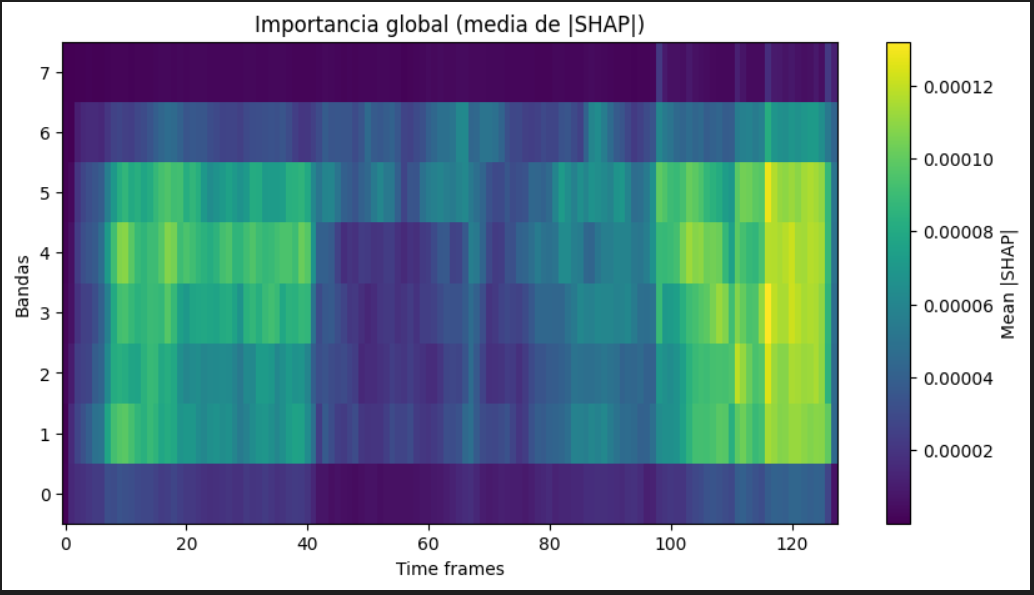
\includegraphics[width=\textwidth]{imagenes/shap_global_espectrogramas_wav2vec2.png}
	\caption{Shap general de los espectrogramas}
	\label{fig:Wav2Vec2}
\end{figure}

En esta imagen sobre la influencia global del shap podemos ver como las partes que más influyen en la clasificación del audio son el principio y el final del audio. Comparando esta gráfica con la anterior podemos confirmar la importancia que tienen las bandas de mel medias. También podemos ver como el audio elegido para la explicación global no es representativo de la explicación global ya que esta última si que usa mucho la parte final del audio para la explicación.

LIME

\begin{figure}[H]
    \centering
    \begin{subfigure}[t]{0.45\textwidth}
        \centering
        
\includegraphics[width=\linewidth]{lime_espectrogramas_wav2vec2.png}
        \caption{Lime de un audio.}
        \end{subfigure}
    \hfill
    \begin{subfigure}[t]{0.45\textwidth}
        \centering
        
\includegraphics[width=\linewidth]{espectrograma_audio.png}
        \caption{Espectrograma de un audio.}
    \end{subfigure}
\end{figure}

En esta imagen se muestra la explicación local de lime sobre mismo audio que en el shap. En ella podemos ver como, al igual que en el shap, las bandas medias son las más relevantes y la pronunciación final es lo que más mueve la predicción hacia la clase real. Por último podemos ver como en estas bandas medias al principio estas empujan la predicción hacia generado, esto se puede deber a que el audio tarda en comenzar y a como pronuncia el principio de la primera palabra ``what''.

\begin{figure}[H]
	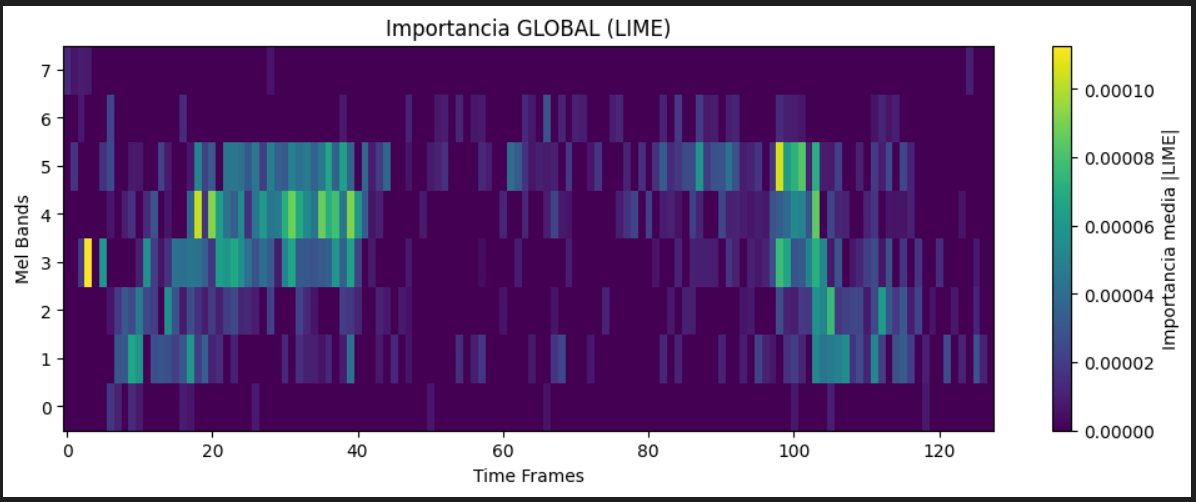
\includegraphics[width=\textwidth]{imagenes/lime_global_espectrogramas_wav2vec2.png}
	\caption{Lime general de los espectrogramas}
	\label{fig:Wav2Vec2}
\end{figure}

Aquí a diferencia de en shap, según lime, el modelo toma las decisiones principalmente gracias al principio de los audios aunque el final también tiene algo de influencia.

INTEGRATED GRADIENTS

\begin{figure}[H]
    \centering
    \begin{subfigure}[t]{0.45\textwidth}
        \centering
        
\includegraphics[width=\linewidth]{ig_espectrogramas_wav2vec2.png}
        \caption{Lime de un audio.}
        \end{subfigure}
    \hfill
    \begin{subfigure}[t]{0.45\textwidth}
        \centering
        
\includegraphics[width=\linewidth]{espectrograma_audio.png}
        \caption{Espectrograma de un audio.}
    \end{subfigure}
\end{figure}

Aquí podemos ver como no está analizando el audio del todo bien ya que las partes más rojas son las que más influyes a una predicción hacia generado pero si vemos el espectrograma del audio, en esas partes como tal no hay nada, son zonas negras, también la gran zona azul del final se corresponde con la parte donde no hay ni siquiera espectrograma. Si ignoramos esas partes y nos centramos solo donde si que hay evidencia de audio, podemos ver como esas son zonas más blancas - azuladas que empujan la predicción hacia real. También se ve como los dos golpes de audio más fuertes en el espectrograma son las partes que más empujan la predicción hacia real.

\begin{figure}[H]
	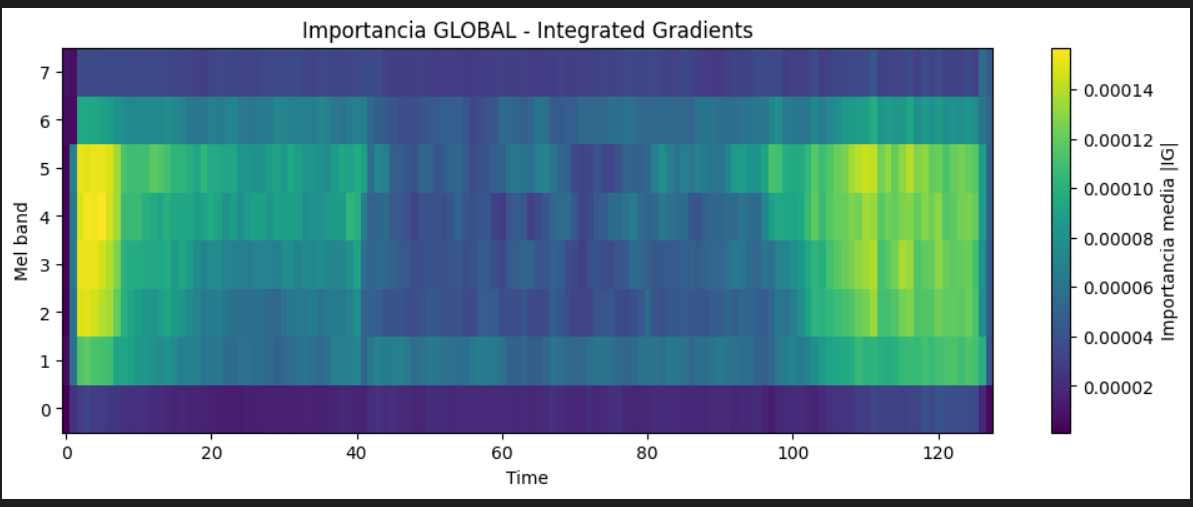
\includegraphics[width=\textwidth]{imagenes/ig_global_espectrogramas_wav2vec2.png}
	\caption{Integrated gradients general de los espectrogramas}
	\label{fig:Wav2Vec2}
\end{figure}

En la predicción global se puede apreciar cierta similitud con las dos explicaciones generales anteriores donde las principales zonas de influencia en la clasificación son la parte inicial y la parte final de los audios en las bandas medias.

GRAD CAM

\begin{figure}[H]
    \centering
    \begin{subfigure}[t]{0.45\textwidth}
        \centering
        
\includegraphics[width=\linewidth]{gc_espectrogramas_wav2vec2.png}
        \caption{Lime de un audio.}
        \end{subfigure}
    \hfill
    \begin{subfigure}[t]{0.45\textwidth}
        \centering
        
\includegraphics[width=\linewidth]{espectrograma_audio.png}
        \caption{Espectrograma de un audio.}
    \end{subfigure}
\end{figure}

Aquí, al igual que en la explicación local de integrated gradients, podemos ver que en las partes donde no hay audio son las partes que más influyen en la predicción aunque aquí si que distingue bien que la parte final donde no hay espectrograma no tiene ningún peso en la predicción. De todas formas, fijándonos donde hay audio podemos apreciar como el primer golpe de voz y la parte final del audio tienen más influencia en la predicción que el resto del mismo.

\begin{figure}[H]
	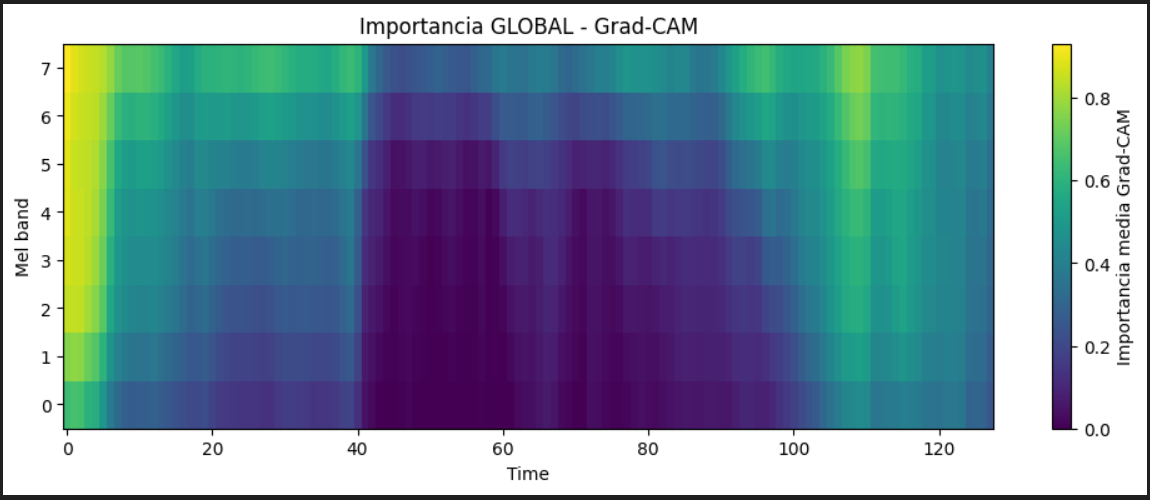
\includegraphics[width=\textwidth]{imagenes/gc_global_espectrogramas_wav2vec2.png}
	\caption{Grad cam general de los espectrogramas}
	\label{fig:Wav2Vec2}
\end{figure}

La explicación global del grad cam se caracteriza por darle el mayor peso a los instantes iniciales del espectrograma, dándole un peso prácticamente nulo al centro del espectrograma, curiosamente donde están los audios, y otorgándole un peso relevante también al final del espectrograma.

Ahora vamos a ver como se ve la agregación de los cuatro modelos de XAI sobre los espectrogramas. Esto se ha calculado para cada frame del espectrograma, se ha sacado su valor en cada una de las explicaciones globales de los distintos modelos y se ha hecho la media aritmética sobre ellos. Antes de poder hacer esto, hemos tenido que normalizar todos las explicaciones ya que estaban en diferentes escalas.

\begin{figure}[H]
	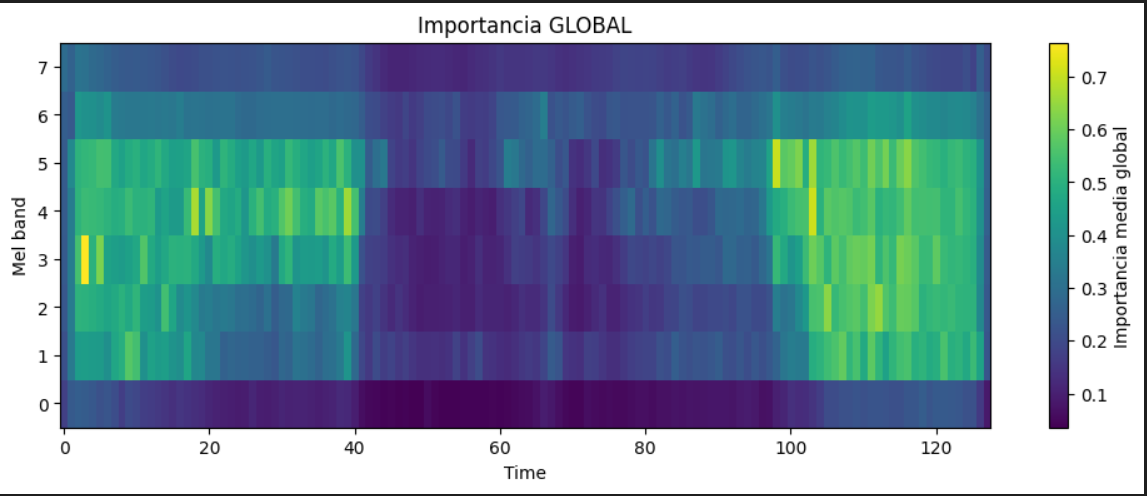
\includegraphics[width=\textwidth]{imagenes/influencia_global_espectrogramas_wav2vec2.png}
	\caption{Lime general de los espectrogramas}
	\label{fig:Wav2Vec2}
\end{figure}

La agregación de las explicaciones globales nos deja claro donde se encuentran las zonas más influyentes siendo el principio y el final del espectrograma dejando al centro con un peso mucho menos relevante.

Como conclusiones podemos sacar que a la vista de los modelos de explicación, parece que el modelo Wav2Vec2 se fija más en los alrededores del audio que en el audio en sí mismo. Esto puede explicartes gracias a las siguitentes propiedades de los espectrogramas de voz:

\begin{enumerate}

 \item Coarticulación: Este es un fenómeno típico de la voz humana donde esta no esta formada por unidades aisladas, es decir, cada sonido depende de los anteriores y posteriores. Esto hace que las transiciones entre fonemas contengan más información que el fonema en sí haciendo que lo que está alrededor del audio tenga más peso.
 
 \item Dinámica espectro-temporal: Las partes centrales de los audios tienden a ser más estables y redundantes mientras que las zonas de cambio contienen mayor variabilidad lo que hace que contengan la mayoría de la información discriminativa del audio.
 
 \item Estructura de formantes y transiciones: Las trayectorias de las formantes, claves para identificar fonemas, suelen estar en los bordes de los segmentos por lo que las zonas de alrededor del audio contienen más información 	dinámica de las formantes.
 
 \item Efectos de ventana del espectrograma: Como el espectrograma se calcula usando ventanas, cada punto del espectrograma mezcla información de un intervalo temporal siendo que en los bordes del espectrograma se incluyen partes de dos sonidos distintos haciendo que estos sean más informativos al incluir mezclas de contextos.
 
 \item Relación señal-ruido: En muchos audios el inicio y el final de los mismos pueden tener cambios de energía o ruido de fondo que el modelo puede usar como señales útiles.
 
 \item Información prosódica: Los elementos como la entonación, el ritmo o el énfasis no están concentrados en un punto sino que ocurren durante las transiciones.

\end{enumerate}